\documentclass[11pt,reqno]{amsart}

\usepackage{amsmath,amssymb,amsthm}
\usepackage{tikz}
\usetikzlibrary{shapes.geometric, positioning, arrows.meta}
\usepackage{tikz-cd}
\usepackage[hidelinks]{hyperref}

\allowdisplaybreaks
\raggedbottom

\newtheorem{theorem}{Theorem}[section]
\newtheorem{proposition}[theorem]{Proposition}
\newtheorem{lemma}[theorem]{Lemma}
\newtheorem{corollary}[theorem]{Corollary}
\theoremstyle{definition}
\newtheorem{definition}[theorem]{Definition}
\newtheorem{openproblem}[theorem]{Open Problem}
\theoremstyle{remark}
\newtheorem{remark}[theorem]{Remark}

\title[Forced noninjectivity in canonical localization]{Forced noninjectivity and infinite sheet resolution in canonical localization}
\author{Matthew Robert Wesney}
\date{Draft of 2026-07-27}

\begin{document}

\begin{abstract}
Kahn's localization construction for $\psi$-polynomial-like maps produces,
at every renormalization stage, a localized inclusion between marked
covers.  The construction is functorial and preserves immersions; the
sources never assert that it preserves embeddings.  We prove that at every
primitively renormalizable ordinary quadratic-like restriction of a
quadratic polynomial (period $p>1$),
the canonically localized inclusion is \emph{forced} to be noninjective:
the degree budget $2^{p}$ against central degree $2$ produces an excess
component of the pulled central continuum, and a peripheral loop around it
lies outside the source localization subgroup while dying in the target.
The failure is resolved canonically: the localized inclusion factors
uniquely (within the based commuting intermediate-cover class) as a
covering onto an embedded intermediate cover, the fiber of
the covering is a pointed coset set, and this sheet defect is
\emph{infinite}, so no finite sheet enumeration is complete.  In fact
the defect has a canonical group model --- the kernel of the
source-to-target hole-filling homomorphism --- and this kernel
surjects, by peripheral winding numbers, onto $\mathbb Z^{\,2^{p}-2}$,
where $2^{p}-2$ is the elementary degree budget of $F=f^{p}$ against
central degree $2$: canonical localization forgets a hole-filling
kernel with exponentially many independent peripheral directions.  The
novelty claimed here is the winding surjection and the kernel
identification, not the count.  The
resolution propagates through Kahn's exact pullback towers on the full,
unselected complementary-cover locus, and
--- under an explicit strong stage-alignment hypothesis --- to the Kahn--Lyubich
direct-decoration depths, where it forces noninjectivity of the induced
tile lifts and of the glued pseudo-piece immersion.  Finally, the infinite
canonical resolution is incompatible with any whole boundary-extended
Kahn--Lyubich tile factorization satisfying the stated annular-tower
typing: an end-compatible comparison of that type forces a
trivial deck kernel.  Two abstract counterexamples (an exactly certified
Blaschke quotient for Kahn's annulus hypotheses, and a complete abstract
$\psi$-quadratic-like pair with a remote self-collision) show that no
argument from the stated hypotheses alone can restore injectivity.  These
results correct an embedding-preservation route proposed in the author's
research program, not in the sources: they contradict
nothing stated in the published sources, and they do not by themselves
decide any global rigidity statement.  The corrective conclusion is
structural: the canonical localized object at an ordinary primitive
canonical seed is not an
embedded pseudo-piece but an embedded cover \emph{together with} an
infinite coset-valued sheet fibration and its canonical transport.
\end{abstract}

\maketitle
\tableofcontents

%=====================================================================
\section{Introduction}\label{sec:intro}

\subsection{Setting}
Renormalization of quadratic-like maps \cite{DH85}, in the generality
needed for
a priori bounds, takes place in Kahn's category of
$\psi$-polynomial-like maps \cite{KahnPrimitive06}: pairs $(i,f)$ of a
holomorphic \emph{immersion} and a proper branched covering between
disks, with a common connected filled preimage.  A central device of
\cite{KahnPrimitive06}, used again in the Kahn--Lyubich decoration
papers \cite{KLDecorations08,KLPrincipal09}, is \emph{localization}: passing to marked
covers determined by the fundamental group of a neighborhood of a marked
full continuum, so that the dynamics near one small filled Julia set can
be studied with the rest of the cycle removed.  Canonical
renormalization is the dynamical localization of the $p$-th iterate at
the central small filled Julia set $A=K_p$, with the cycle
$B=\mathcal K_p$ removed.

The sources are careful about what this construction preserves.  The
localization functor preserves immersions and branched coverings; the
localized inclusion leg is asserted to be an immersion, never an
embedding; and Kahn notes explicitly that the map which was an embedding
in the quadratic-like setting has become an immersion in the
$\psi$-quadratic-like setting.  We are not aware of any statement in
the literature determining whether this caution is necessary at the
canonical stages themselves --- whether the canonically localized
inclusion might in fact be injective, so that localization could be
treated as embedding-preserving in arguments that need a globally
embedded local model.  Section~\ref{subsec:literature} records what we
did examine and what the closest published anticipation is.

\subsection{Main results}
We show that the caution is necessary in the strongest possible sense:
noninjectivity is not merely possible but \emph{forced}, at every
ordinary primitive canonical seed, and the failure carries a canonical
infinite structure.

Throughout, $f\colon U^{1}\to U^{0}$ is an ordinary quadratic-like
restriction of a quadratic polynomial, primitively renormalizable of
period $p>1$; $F=f^{p}\colon U^{p}\to U^{0}$; $A=K_{p}$ is the central
small filled Julia set and $B=\mathcal K_{p}$ its cycle;
$T'=(U^{p}\setminus F^{-1}B)\cup A$ and $T=(U^{0}\setminus B)\cup A$ are
the marked surfaces of Kahn's canonical localization, with localization
subgroups $H_{s}\le\pi_{1}(T'\setminus A)$ and
$H_{t}\le\pi_{1}(T\setminus A)$, localization covers
$\widehat\Omega_{s}$ and $\widehat\Omega_{t}$ of the complementary
surfaces $\Omega_{s}=T'\setminus A$ and $\Omega_{t}=T\setminus A$,
complement-cover lift
$\widehat a\colon\widehat\Omega_{s}\to\widehat\Omega_{t}$, and localized
inclusion $\widehat\imath\colon T'_{A}\to T_{A}$.

\begin{theorem}[Forced noninjectivity; Theorem~\ref{thm:forced-collision}]
\label{thm:A}
At every ordinary primitive canonical seed of period $p>1$, the
canonically localized inclusion $\widehat\imath$ is not injective.
Explicitly, there are an excess component $X\neq A$ of $F^{-1}(A)$ and a
based loop $\gamma\subset U^{p}\setminus F^{-1}B$ with
$[\gamma]\notin H_{s}$ and $(i^{p})_{*}[\gamma]=1\in H_{t}$, and the
lift of $\gamma$ has distinct endpoints identified by
$\widehat\imath$.
\end{theorem}

\begin{theorem}[Canonical resolution; Theorems~\ref{thm:sheet-resolution}
and~\ref{thm:unique-intermediate}]\label{thm:B}
The complement-cover lift $\widehat a$ of $i^{p}$ factors exactly as
$\widehat a=e\circ q$, where
$q\colon\widehat\Omega_{s}\to P_{K}$ is a surjective covering onto the
basepoint component $P_{K}$ of the corresponding pullback cover and
$e\colon P_{K}\hookrightarrow\widehat\Omega_{t}$ is a topological
embedding.  Every point collision of $\widehat\imath$ lies in the
complement-cover part, where $\widehat\imath$ agrees with $\widehat a$,
and is a sheet identification of $q$; the
based fiber of $q$ is the pointed coset set $K/H_{s}$ with
$K=(i^{p})_{*}^{-1}(H_{t})$ the reflected subgroup; and $P_{K}$ is the
unique connected intermediate cover, in the based commuting comparison
class of Theorem~\ref{thm:unique-intermediate}, on which the remaining
leg embeds.  No extension of the factorization across the filled
completion is asserted.
\end{theorem}

\begin{remark}[The structural shape of Theorem~\ref{thm:B} is not new]
\label{rem:covering-embedding-prior}
The shape asserted by Theorem~\ref{thm:B} --- an immersion that is a
covering onto an embedded image away from a proper compactum --- is
already an axiomatised notion in the recent literature.
Dudko--Luo--Lyubich \cite[\S2.1]{DLL25} call an immersion
$\iota\colon A\to B$ a \emph{covering embedding rel $S\subset B$} when
$S$ is $\iota$-proper and $\iota$ restricted to
$A\setminus\iota^{-1}(S)$ is a covering onto its image, and they impose
this as Items (V)--(VI) of their $\psi$-ql Siegel definition.  Their
setting is different (Siegel rather than primitive) and, decisively,
the property is \emph{imposed} there as part of a definition.  The
contribution of Theorem~\ref{thm:B} is not the notion but its
canonical derivation at the seed: the factorization is produced,
its intermediate factor is shown to be unique in a stated comparison
class, and its fiber is identified with an explicit dynamical coset
set.
\end{remark}

\begin{theorem}[Infinite sheet defect;
Corollary~\ref{cor:infinite-defect}]\label{thm:C}
At every ordinary primitive canonical seed, $[K:H_{s}]=\infty$:
the cosets $[\gamma]^{n}H_{s}$ are pairwise distinct.  Consequently
every non-singleton fiber of $\widehat\imath$ (equivalently, every
fiber over the embedded resolved complement component) is infinite and
no finite raw
sheet enumeration of the canonical localization is complete.
\end{theorem}

\begin{theorem}[Kernel normal form;
Theorem~\ref{thm:kernel-normal-form}]\label{thm:Cprime}
At every ordinary primitive canonical seed, with the shared local
neighborhood and based subgroup representatives of
Definition~\ref{def:shared-neighborhood}, the hole-filling
homomorphism $a_{*}=(i^{p})_{*}$ restricts to an isomorphism
$H_{s}\to H_{t}$, and the reflected subgroup splits as
$K=N_{\mathrm{fill}}\rtimes H_{s}$ with
$N_{\mathrm{fill}}=\ker a_{*}$.  Consequently $n\mapsto nH_{s}$ is a
canonical pointed bijection $N_{\mathrm{fill}}\to K/H_{s}$: the sheet
fiber carries a canonical group model, and canonical localization
forgets exactly the kernel of the source-to-target hole-filling map.
\end{theorem}

\begin{theorem}[Exact excess count and exponential defect;
Theorem~\ref{thm:excess-count},
Corollary~\ref{cor:exponential-defect}]\label{thm:Cpp}
At every ordinary primitive canonical seed of period $p>1$ the central
preimage decomposes as
$F^{-1}(A)=A\sqcup X_{1}\sqcup\cdots\sqcup X_{2^{p}-2}$, where each
excess component $X_{j}$ is a full continuum disjoint from $B$ mapped
homeomorphically onto $A$ by $F$.  The peripheral winding vector about
the excess components is a surjective homomorphism
$N_{\mathrm{fill}}\twoheadrightarrow\mathbb Z^{\,2^{p}-2}$; hence
$\operatorname{rank}H_{1}(N_{\mathrm{fill}};\mathbb Z)\ge 2^{p}-2$,
and the forgotten sheet fiber carries at least $2^{p}-2$ independent
peripheral winding coordinates.
\end{theorem}

Two calibrations of Theorem~\ref{thm:Cpp}.  The count $2^{p}-2$ is an
elementary degree budget --- $\deg F=2^{p}$, the only critical point of
$F$ whose critical value lies in $A$ is the origin, so every other
component of $F^{-1}(A)$ is univalent --- and we claim no novelty for
it; the existence of non-central components is in any case structurally
built into the hypothesis of the Kahn--Lyubich Covering Lemma
(\cite[\S4]{KLDecorations08}: $A$ is a component of $f^{-1}(B)$ with
big degree $D$ and local degree $d$, and $D>d$ forces further
components).  What is claimed is the peripheral-winding surjection
$N_{\mathrm{fill}}\twoheadrightarrow\mathbb Z^{\,2^{p}-2}$ and the
resulting rank bound.  Likewise, the abstract covering-space
factorization is standard; the contribution is the identification of
the actual dynamical subgroup defect and its canonical kernel model,
not the invention of intermediate covers.

\begin{theorem}[Exact propagation; Proposition~\ref{prop:base-change},
Corollary~\ref{cor:kahn-tower}, Theorem~\ref{thm:propagation}]\label{thm:D}
The factorization and its fiber data are preserved by every full,
unselected exact Kahn equalizer on the complementary-cover locus, hence
by every depth of Kahn's pullback iteration of the same seed.  Under
the strong stage-alignment hypothesis
(Definition~\ref{def:strong-alignment}), the
collision transports to the exact decoration depths
$m=\nu q+1$, $n=(\nu-1)q+1$, where it forces noninjectivity of the
Kahn--Lyubich ambient annulus arrow, of every compatible full
universal-cover tile lift, and of the full glued pseudo-piece
immersion.
\end{theorem}

\begin{theorem}[No aligned annular realization of the canonical
infinite resolution is a whole KL tile;
Theorem~\ref{thm:whole-tile-no-go},
Corollary~\ref{cor:canonical-not-whole-tile}]\label{thm:E}
Whenever the canonical resolved factorization restricts, at an aligned
stage, to a covering/embedding factorization of a degree-one immersion
of finite-modulus annuli, the full annular-tower typing of
Definition~\ref{def:canonical-resolved-system} is automatic
(Theorem~\ref{thm:annular-normal-form}), and no end-compatible
whole-tile comparison square can identify the
canonical resolved factorization with a complete boundary-extended
Kahn--Lyubich tile factorization carrying the two source-locked
infinitely-wrapping vertices: any such comparison forces the deck
kernel to be trivial, while the canonical resolution has infinite
sheet defect.  The statement is conditional only on the aligned-stage
annular factorization; the typing is derived, not assumed.
\end{theorem}

Two abstract counterexamples calibrate the main theorems.  A degree-one
annular immersion satisfying all stated hypotheses of Kahn's annulus
lemma can fail to be injective (Theorem~\ref{thm:annulus-nogo}; an
exactly certified Blaschke quotient), and the complete abstract
$\psi$-quadratic-like axioms admit a pair whose immersion has an
explicit remote self-collision (Theorem~\ref{thm:psiql-nogo}).  Thus no
proof from the stated hypotheses alone --- degree, immersion,
properness of the companion branch, common connected inverse --- can
restore global injectivity; the forced collision of
Theorem~\ref{thm:A} is a fact about the actual dynamical construction,
established by the actual excess-component geometry.

\subsection{Relation to the literature}
\label{subsec:literature}
Because the results above are stated against two specific sources, we
record what was examined, what the closest published anticipation is,
and how much of the argument is short once one knows to look for it.

\emph{What the primary sources assert.}  Kahn's localization functor is
asserted to preserve immersions and branched coverings and nothing more
(\cite[\S\S7.4.1--7.4.2, pp.~43--45]{KahnPrimitive06}); at the
quadratic-like stage the arrow $i$ is literally the inclusion of nested
domains, and a footnote announces that in the $\psi$-quadratic-like
sections it will be replaced by an immersion
(\cite[\S6, p.~31 and footnote 15]{KahnPrimitive06}); and the setup
ingredient of the present argument is already visible in the source, since
\cite[\S6.1, pp.~31--32]{KahnPrimitive06} exhibits the hole-filling leg
$U^{n+1}\setminus f^{-1}\mathcal K\subset U^{n+1}\setminus\mathcal K$ as
one side of a triangle the text explicitly calls non-commutative, and
controls passage along it quantitatively via Property~D.  On the
Kahn--Lyubich side the pseudo-piece inclusion arrow is never upgraded
beyond an immersion \cite[\S3.2.2, Lemma~3.4]{KLDecorations08}.

\emph{The closest published anticipation.}  It is by the source authors
themselves, and it deserves to be in the introduction rather than in an
appendix.  In the proof of \cite[\S3.2.2, Lemma~3.4(ii), p.~68 of the
journal pagination]{KLDecorations08}, for puzzle pieces $Y\subset Z$ the
components $Y_{i}$ are embedded into components $Z_{j(i)}$, and the
component index map $j=j(i)$ is described as ``surjective but not
necessarily injective''.  That is the collapsing-of-components
mechanism, in print, since 2008.  Theorem~\ref{thm:A} differs from it in
three specific ways.
\begin{enumerate}
\item[(1)] It is a \emph{forcing} statement, not a possibility
  statement: at every ordinary primitive canonical seed the collision
  must occur, whereas ``not necessarily injective'' asserts only that
  injectivity is not guaranteed.
\item[(2)] It concerns the \emph{glued immersion}, not the component
  index map $j$.  Noninjectivity of $j$ does not imply noninjectivity of
  the glued map: distinct universal-cover tiles can occupy disjoint
  sheets over one target tile, so a two-to-one $j$ is compatible with
  an injective glued arrow.
\item[(3)] It concerns Kahn's localization functor at a canonical
  \emph{seed}, not Kahn--Lyubich pseudo-puzzle tiles at an arbitrary
  puzzle depth.
\end{enumerate}

\emph{On difficulty.}  We do not present Theorem~\ref{thm:A} as hard.
In Kahn's own path model of the canonical localization
(\cite[\S7.4.5, pp.~46--47]{KahnPrimitive06}), where the source class
space is formed rel $f^{-p}(K_{p})$ and the target rel $\mathcal K_{p}$
and the source proves only the forward direction of path equivalence,
the failure of injectivity is a short argument once one thinks to look
for it: a loop around an excess component of
$f^{-p}(K_{p})\setminus\mathcal K_{p}$ is nontrivial in the source
class space and trivial in the target.  We are not aware of anyone
having recorded it, and the substance of this paper lies in what
follows from it --- the kernel normal form, the infinitude
$[K:H_{s}]=\infty$, the rank-$(2^{p}-2)$ winding surjection, and the
propagation and no-go results.

\emph{Post-2008 work on this machinery.}  We examined the papers that
actually use the $\psi$-ql/localization apparatus and found no
statement of, and nothing contradicting, Theorem~\ref{thm:A}.  The most
recent restatement of the construction is by two of the three source
authors: Kahn--Kapiamba--Lyubich \cite[\S\S2.2--2.3]{KKL26} recall
localization via subsurface covers and renormalization, and still
assert only that the pair $(f^{n},\iota^{n})$ \emph{lifts} to a
$\psi$-ql map --- no embedding, injectivity, or sheet statement.  The
same holds in \cite{KLElephant26}, where $\iota$ is used on
complements with no injectivity claim; in the Dudko--Lyubich
renormalization papers \cite{DL22,DL23}; in the Siegel variation
\cite{DLL25}, whose \S2.1 axiomatises the covering-embedding shape
discussed in Remark~\ref{rem:covering-embedding-prior}; in
\cite{CS15}; and in \cite{BLOT22}.  Dudko's survey \cite{Dudko25}
does not treat the localization functor at this level of detail.  We
make no claim of an exhaustive search: the negative result rests on the
citation graphs of the two sources together with targeted full-text
checks, not on a complete bibliographic sweep.

\subsection{What these results do and do not assert}
\label{subsec:scope}
Three boundaries govern everything below and are restated where they
apply.

\emph{First}, the results contradict nothing stated in the published
sources \cite{KahnPrimitive06} and \cite{KLDecorations08}; the exact
identification points on which this interface rests are listed in
Section~\ref{sec:verification}.  Those sources
assert immersion preservation, a homeomorphism on filled and marked
sets, an embedded inner collar, and the forward direction of path
equivalence --- never a global embedding of the localized inclusion.
In particular the embedded inner collar of
\cite[Theorem~7.3, p.~37]{KahnPrimitive06} and
\cite[Lemma~3.1, p.~10]{KLDecorations08} is \emph{not} in tension with
Theorem~\ref{thm:A}: the forced collision is located outside the
collar, on a peripheral loop around an excess component in the outer
part of the source, as spelled out in
Remark~\ref{rem:collar-compat}.  What is refuted is a proposed
\emph{extension} of the sources: any argument treating canonical
localization as embedding-preserving.
Appendix~\ref{sec:disclosures} documents where the sources themselves
demote the inclusion to an immersion.

\emph{Second}, the direct-decoration consequences in
Theorem~\ref{thm:D} are conditional on the strong stage-alignment
hypothesis (Definition~\ref{def:strong-alignment}) for the same
canonical seed; the alignment and realization
quantifiers are stated exactly in Proposition~\ref{prop:realization},
and no source-locked parameter realization is claimed.  As
Remark~\ref{rem:alignment-is-seed-identification} explains, that
hypothesis is not a comparison of two constructions --- the
Kahn--Lyubich ambient arrow is literally an iterate of Kahn's
equalizer tower --- but an identification of two \emph{seeds}: on the
reading this paper intends, in which the Kahn--Lyubich puzzle
machinery is run over the canonical seed itself, the identifications
are the identity and Theorem~\ref{thm:D} is unconditional; it is the
distinct-seed reading that remains open.

\emph{Third}, the results are corrective, not constructive, with
respect to any global program: they show that the full embedded
pseudo-piece cannot be the universal carrier invariant, and that a
valid replacement must retain the coset-valued sheet fibration and its
transport, or synchronize the removed obstacle packet.  They do not by
themselves prove or refute any rigidity, a~priori bounds, or local
connectivity statement, and we make no claim in that direction.

\subsection{Organization}
Section~\ref{sec:background} fixes the $\psi$-polynomial-like
background and the localization construction.  All citations into the
two primary sources are given by published section, statement number
and page; the SHA-256--locked \TeX{} archives on which the paraphrases
were originally prepared are retained only as a provenance concordance
in Appendix~\ref{app:sourcelock}.
Section~\ref{sec:criteria} develops the criterion layer: the
subgroup-reflection criterion and peripheral isolation of pulled full
continua.  Section~\ref{sec:forced} proves
Theorem~\ref{thm:A}; Section~\ref{sec:resolution} proves
Theorems~\ref{thm:B} and~\ref{thm:C} and constructs the sheet-transport
groupoid; Section~\ref{sec:enlargement} gives the exact coset tests for
enlargement.  Section~\ref{sec:kernel} proves
Theorems~\ref{thm:Cprime} and~\ref{thm:Cpp}: the kernel normal form,
the exact excess count, and the exponential winding defect of the
hole-filling kernel.  Section~\ref{sec:basechange} proves the
base-change half
of Theorem~\ref{thm:D}; Section~\ref{sec:tiles} transports the
collision to tiles and pseudo-pieces; Section~\ref{sec:wholetile}
proves Theorem~\ref{thm:E}.  Section~\ref{sec:seedvsbold} separates the
ordinary canonical seed from a general bold Kahn--Lyubich stage.
Section~\ref{sec:changes} states what these results change in
localization arguments.  Section~\ref{sec:verification} records the
outcome of the source check on the identifications on which the
interface with the sources rests, together with the exact scope of the
machine-checked certificates.  Appendix~\ref{sec:disclosures} collects
the annulus immersion lemma and the sources' immersion disclosures;
Appendix~\ref{sec:abstract} gives the
two abstract counterexamples.  Appendix~\ref{app:certificates} records
the certificate conventions; Appendix~\ref{app:sourcelock} records the
source-lock data.

\subsection*{Provenance and verification disclosure}
This paper was prepared with extensive machine assistance, both in the
research phase and in drafting, within a source-locked, machine-audited
research framework; the supporting dependency ledger and validation
scripts are available with the manuscript sources.  The
machine-verified content is strictly delimited (exact rational
certificates for Appendix~\ref{sec:abstract}; source-lock hashes;
arithmetic and routing checks) and is described in
Section~\ref{sec:verification}.  We stand behind the unconditional
core of the paper --- the forced collision, the canonical resolution,
the kernel normal form, and the exact excess count.  The Kahn-side
identifications on which that core rests have now been checked against
the published sources and are recorded as confirmed, with their
published loci, in Section~\ref{sec:verification}; specialist
confirmation is invited but the checks are no longer unperformed.  The
Kahn--Lyubich consequences are stated as precise implications under
the strong stage-alignment hypothesis
(Definition~\ref{def:strong-alignment}), whose real content ---
identifying two seeds, not two constructions --- is analysed in
Remark~\ref{rem:alignment-is-seed-identification}.  On the reading
this paper intends, in which the Kahn--Lyubich puzzle machinery is run
over the canonical seed itself, those consequences are unconditional;
supplying the identifications for a \emph{different} seed is the one
source-side proposition that remains open.

%=====================================================================
\section{Background: $\psi$-polynomial-like maps and localization}
\label{sec:background}

This section fixes definitions and records, in paraphrase, exactly what
the published sources provide.  Citations read
``Kahn~I, \S X / Theorem~N, p.~P'' for
\cite{KahnPrimitive06} in the numbering of arXiv:math/0609045v3
(28 December 2023, 63 pp.), and ``KL~II, Lemma~N, p.~P'' for
\cite{KLDecorations08} in the numbering of
Ann.\ Sci.\ \'Ec.\ Norm.\ Sup\'er.\ (4) \textbf{41} (2008) 57--84 and
of the identically sectioned arXiv:math/0609046v2.  The SHA-256--locked
\TeX{} archives from which the paraphrases were prepared, and their
concordance to these published loci, are recorded in
Appendix~\ref{app:sourcelock}.

\emph{Path convention.}  For paths $\alpha,\beta$ with
$\alpha(1)=\beta(0)$, the concatenation $\alpha*\beta$ traverses
$\alpha$ first.  All displayed loop products below use this
convention.

%%INSERT F:notation
%%INSERT F:definitions

Beyond the definitions, the body of the paper uses five statements of
the sources, each a paraphrase with published citations: the
polynomial-like restriction theorem, the exact pullback tower, the
localization theorem, dynamical localization, and canonical
renormalization.  Kahn's annulus immersion lemma and the four source
passages demoting the localized inclusion from an embedding to an
immersion are needed only for calibration and scope; they are
collected, under the same citation conventions, in
Appendix~\ref{sec:disclosures}.

%%INSERT F:thm_01
%%INSERT F:thm_02
%%INSERT F:thm_03
%%INSERT F:thm_04
%%INSERT F:thm_05

\subsection*{Calibration by two abstract counterexamples}
Two abstract counterexamples calibrate everything that follows: an
exactly certified Blaschke quotient shows Kahn's annulus hypotheses
alone do not imply global injectivity, and a complete abstract
$\psi$-quadratic-like pair exhibits a remote self-collision
(Appendix~\ref{sec:abstract}).  After those examples, any injectivity
assertion for an actual localized inclusion must use its dynamical
construction history; the body of this paper shows the canonical
answer is negative for dynamical reasons.

%=====================================================================
\section{The criterion layer}
\label{sec:criteria}

The forced collision of Section~\ref{sec:forced} is proved against two
pieces of infrastructure: an exact covering-space criterion measuring
when a localized lift is injective, and a finite-topology toolkit
isolating pulled full continua.  Both are elementary; both are stated
and proved in full because the direction of every subgroup inclusion is
load-bearing later.

\subsection{The subgroup-reflection criterion}
%%INSERT B:notation
%%INSERT B:definitions
%%INSERT B:thm_00
%%INSERT B:thm_01
%%INSERT B:thm_02

\subsection{Peripheral isolation of pulled full continua}
%%INSERT C:notation
%%INSERT C:definitions
%%INSERT C:thm_00
%%INSERT C:thm_01
%%INSERT C:thm_02
%%INSERT C:thm_03
%%INSERT C:thm_04

%=====================================================================
\section{Forced noninjectivity at ordinary primitive canonical seeds}
\label{sec:forced}

\begin{figure}[t]
\centering
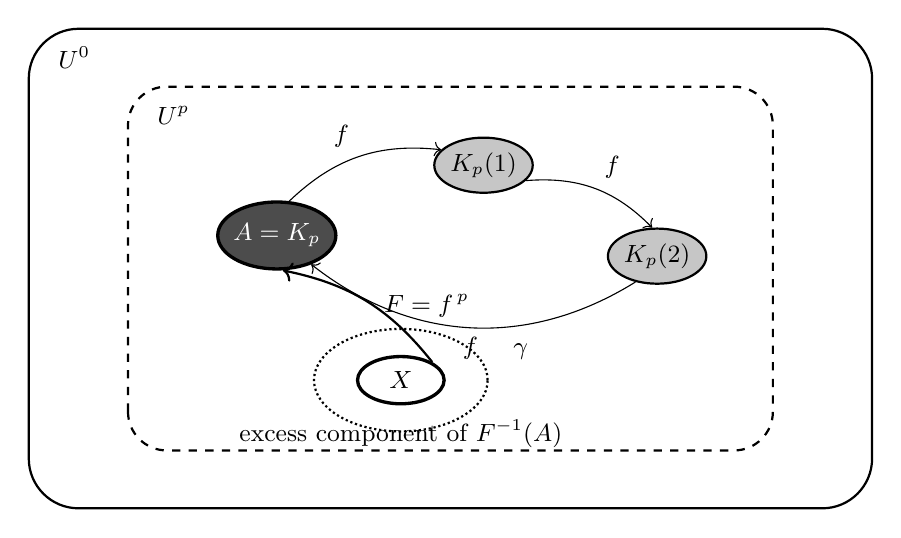
\begin{tikzpicture}[scale=1.05,
  blob/.style={draw, thick, fill=gray!12, rounded corners=6pt},
  julia/.style={draw, thick, fill=gray!45},
  juliaA/.style={draw, very thick, fill=black!70},
  lbl/.style={font=\small}]
  % ambient U^0
  \draw[thick, rounded corners=18pt] (-5.1,-2.9) rectangle (5.1,2.9);
  \node[lbl] at (-4.55,2.55) {\(U^{0}\)};
  % U^p
  \draw[thick, dashed, rounded corners=14pt] (-3.9,-2.2) rectangle (3.9,2.2);
  \node[lbl] at (-3.35,1.85) {\(U^{p}\)};
  % the cycle B = K_p(0) u ... u K_p(p-1), p = 3, with A = K_p = K_p(0)
  \node[juliaA, ellipse, minimum width=1.5cm, minimum height=0.85cm] (A) at (-2.1,0.4) {};
  \node[lbl, white] at (A) {\(A=K_p\)};
  \node[julia, ellipse, minimum width=1.25cm, minimum height=0.7cm] (K1) at (0.4,1.25) {};
  \node[lbl] at (0.4,1.25) {\(K_p(1)\)};
  \node[julia, ellipse, minimum width=1.25cm, minimum height=0.7cm] (K2) at (2.5,0.15) {};
  \node[lbl] at (2.5,0.15) {\(K_p(2)\)};
  % cycle arrows under f
  \draw[->, bend left=25] (A.70) to node[lbl, above left] {\(f\)} (K1.160);
  \draw[->, bend left=25] (K1.-20) to node[lbl, above right] {\(f\)} (K2.100);
  \draw[->, bend left=35] (K2.-130) to node[lbl, below] {\(f\)} (A.-40);
  % excess component X of F^{-1}(A)
  \node[draw, very thick, fill=white, ellipse, minimum width=1.1cm, minimum height=0.6cm]
    (X) at (-0.6,-1.35) {};
  \node[lbl] at (-0.6,-1.35) {\(X\)};
  \node[lbl] at (-0.6,-2.0) {excess component of \(F^{-1}(A)\)};
  \draw[->, bend right=20, thick] (X.30) to node[lbl, right, pos=0.45] {\(F=f^{\,p}\)} (A.-80);
  % the based loop gamma around X
  \draw[thick, densely dotted] (-0.6,-1.35) ellipse (1.05cm and 0.62cm);
  \node[lbl] at (0.85,-1.0) {\(\gamma\)};
\end{tikzpicture}
\caption{The canonical seed of a primitive renormalization of period \(p\)
(drawn for \(p=3\)).  The cycle
\(B=\mathcal K_p=\bigcup_{j}K_p(j)\) is removed and the central continuum
\(A=K_p\) is retained on both sides.  Because \(\deg F=2^{p}\) exceeds the
central degree \(2\), the preimage \(F^{-1}(A)\) has a component
\(X\neq A\).  A based loop \(\gamma\) encircling \(X\) lies outside the
source localization subgroup but is contracted by the physical inclusion in
the target: its localized lift has distinct endpoints that the localized
inclusion identifies.}
\label{fig:seed}
\end{figure}
\begin{figure}[t]
\centering
\begin{tikzcd}[row sep=large, column sep=huge]
  T'_{A}
    \arrow[r, "\widehat{\imath}"]
    \arrow[d, "\pi_{s}"']
  & T_{A}
    \arrow[d, "\pi_{t}"]
  \\
  T' = (U^{p}\setminus F^{-1}B)\cup A
    \arrow[r, hook, "i^{p}"']
  & T = (U^{0}\setminus B)\cup A
\end{tikzcd}
\caption{The localization covers.  The covers \(\pi_{s},\pi_{t}\) are the
based covers classified by the localization subgroups
\(H_{s}\le\pi_{1}(T'\setminus A)\) and \(H_{t}\le\pi_{1}(T\setminus A)\); the localized inclusion
\(\widehat{\imath}\) is the unique based lift of the physical inclusion
\(i^{p}\).  The forced collision is the statement that
\(\widehat{\imath}\) is never injective at an ordinary primitive canonical
seed of period \(p>1\): the class \([\gamma]\) of
Figure~\ref{fig:seed} lies outside \(H_{s}\) while
\((i^{p})_{*}[\gamma]\) is trivial in \(H_{t}\).}
\label{fig:covers}
\end{figure}

This section proves Theorem~\ref{thm:A}.  The mechanism is summarized
by Figures~\ref{fig:seed} and~\ref{fig:covers}: the degree budget
produces an excess component $X$ of $F^{-1}(A)$; peripheral isolation
puts an isolating Jordan disk around $X$; the winding number about $X$
defines a homomorphism killing the source localization subgroup but not
the peripheral class; and the target contracts the peripheral loop
across the isolating disk, since the target removes only $B$ while the
source removes all of $F^{-1}B$.

% New lemmas addressing review items A, B, and the completion step.

\begin{lemma}[Jordan neighborhoods are local pairs]\label{lem:local-pair}
Let $A\subset\mathbb C$ be a nondegenerate full continuum compactly
contained in a Jordan disk $D_A$.  Then $D_A\setminus A$ is a
topological annulus; in particular $(D_A,A)$ is a local pair in the
sense of the localization construction
(Definition~\ref{def:localization}).
\end{lemma}

\begin{proof}
A connected component of $D_A\setminus A$ whose closure does not meet
$\partial D_A$ would be a bounded component of $\mathbb C\setminus A$,
contradicting fullness of $A$; hence $D_A\setminus A$ is connected.
In the sphere $\widehat{\mathbb C}$, the complement of $D_A\setminus A$
has exactly the two components $A$ and
$\widehat{\mathbb C}\setminus D_A$, so $D_A\setminus A$ is a doubly
connected plane domain, i.e.\ an annulus.  Its fundamental group is
infinite cyclic, generated by a core curve, which is the defining
property of a local pair.
\end{proof}

\begin{definition}[Shared local neighborhood and based subgroup
representatives]\label{def:shared-neighborhood}
Fix once and for all a Jordan disk $D_A\supset A$ with
$\overline{D_A}\subset U^{p}$ and
$\overline{D_A}\cap\bigl(F^{-1}B\setminus A\bigr)=\varnothing$; such a
disk exists because $F^{-1}B\setminus A$ is a compact set disjoint from
the component $A$ of $F^{-1}B$.  Since
$\Omega_s=T'\setminus A\subset T\setminus A=\Omega_t$ and
$D_A\setminus A\subset\Omega_s$, the same disk is a valid local
neighborhood on both sides.  With a common basepoint and connecting
path fixed in $D_A\setminus A$, define
\[
 H_s=\operatorname{im}\bigl[\pi_1(D_A\setminus A)\to\pi_1(\Omega_s)\bigr],
 \qquad
 H_t=\operatorname{im}\bigl[\pi_1(D_A\setminus A)\to\pi_1(\Omega_t)\bigr].
\]
These are the based representatives of the localization subgroups used
throughout; the collision certificate is representative-independent
(the winding homomorphism kills every conjugate of $H_s$).
\end{definition}

\begin{lemma}[Injectivity of the completion]\label{lem:completion-injective}
In the connected-complement localization construction
(Theorem~\ref{thm:kahn-localization}), the natural map from the
complement covering surface $\widehat\Omega$ into the completed
localized surface $S_A$ is injective.
\end{lemma}

\begin{proof}
The completed surface is the quotient of the disjoint union
$U\sqcup\widehat\Omega$ in which each point $u\in U\setminus A$ is
identified with its image $\ell(u)\in\widehat\Omega$ under the
canonical lift $\ell$ of $U\setminus A$.  Every identification therefore
pairs one point of $U$ with one point of $\widehat\Omega$; no two
points of $\widehat\Omega$ are ever identified with one another, since
$\ell$ is single-valued.  Hence the composition
$\widehat\Omega\hookrightarrow U\sqcup\widehat\Omega\to S_A$ is
injective.
\end{proof}

\begin{remark}\label{rem:completion-consequence}
Lemma~\ref{lem:completion-injective}, applied on both sides, shows that
the filled completion identifies no pair of distinct complement-cover
points.  Consequently every point collision of the completed localized
inclusion $\widehat\imath$ arises from a collision of the
complement-cover lift $\widehat a$, and conversely; this is the bridge
invoked in Theorem~\ref{thm:forced-collision}, now proved rather than
delegated to the verification checklist of
Section~\ref{sec:verification}.
\end{remark}


%%INSERT C:thm_05
%%INSERT C:thm_06
%%INSERT C:thm_07
%%INSERT C:thm_10

%=====================================================================
\section{The canonical sheet resolution and the infinite defect}
\label{sec:resolution}

\begin{figure}[t]
\centering
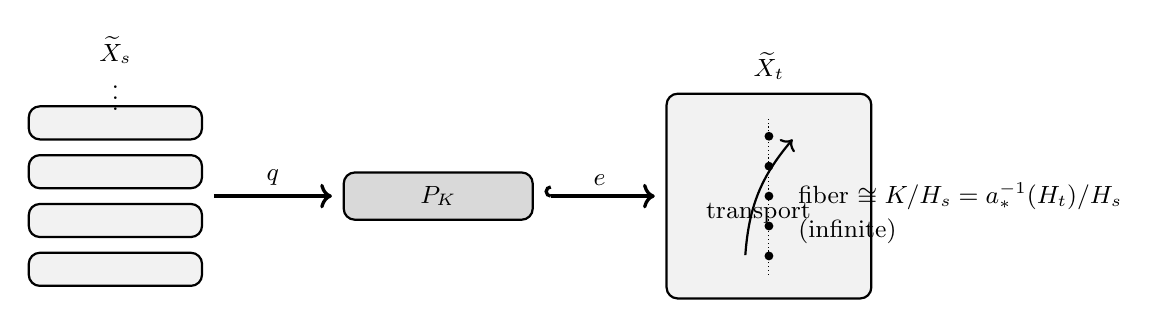
\begin{tikzpicture}[scale=1.0,
  sheet/.style={draw, thick, rounded corners=4pt, fill=gray!10},
  lbl/.style={font=\small}]
  % source resolved cover: stack of sheets
  \foreach \k in {0,1,2,3} {
    \node[sheet, minimum width=2.2cm, minimum height=0.42cm]
      at (-4.1, {0.62*\k - 0.93}) {};
  }
  \node[lbl] at (-4.1, 1.85) {\(\widetilde X_{s}\)};
  \node[lbl] at (-4.1, 1.35) {\(\vdots\)};
  % middle embedded factor P_K
  \node[sheet, fill=gray!30, minimum width=2.4cm, minimum height=0.6cm] (PK) at (0,0) {};
  \node[lbl] at (0, 0) {\(P_{K}\)};
  % target cover
  \node[sheet, minimum width=2.6cm, minimum height=2.6cm] (Xt) at (4.2,0) {};
  \node[lbl] at (4.2, 1.65) {\(\widetilde X_{t}\)};
  % maps
  \draw[->, very thick] (-2.85,0) -- node[lbl, above] {\(q\)} (-1.35,0);
  \draw[{Hooks[right]}->, very thick] (1.35,0) -- node[lbl, above] {\(e\)} (2.75,0);
  % coset fiber column inside X_t
  \foreach \k in {-2,-1,0,1,2} {
    \fill (4.2, {0.38*\k}) circle (1.6pt);
  }
  \draw[densely dotted] (4.2,-1.0) -- (4.2,1.0);
  \node[lbl, right] at (4.45, 0.0) {fiber \(\cong K/H_{s}=a_{*}^{-1}(H_{t})/H_{s}\)};
  \node[lbl, right] at (4.45, -0.45) {(infinite)};
  % transport arrow
  \draw[->, bend left=18, thick] (3.9, -0.75) to node[lbl, below] {transport} (4.5, 0.72);
\end{tikzpicture}
\caption{The canonical intermediate-cover resolution.  The unresolved
immersed pseudo-piece is replaced by the factorization
\(\widetilde X_{s}\xrightarrow{\,q\,}P_{K}\lhook\joinrel\xrightarrow{\,e\,}\widetilde X_{t}\):
a covering onto the embedded intermediate factor (unique in the based
commuting comparison class) followed by an
embedding.  The sheet fiber over the embedded factor is a coset space
detected by the winding homomorphism; it is infinite, and canonical
transport moves sheets along paths in the base.  Exact Kahn base change
preserves the entire structure.}
\label{fig:sheets}
\end{figure}

This section proves Theorems~\ref{thm:B} and~\ref{thm:C}.  The results
are stated for an abstract based embedding $a$ between bases of
connected covers, with based lift $A$.  The factorization is summarized
by Figure~\ref{fig:sheets}.

\emph{Notational scope:} within
Sections~\ref{sec:resolution}--\ref{sec:wholetile} several symbols are
reused in the abstract covering and tile settings, and each is to be
resolved at its local declaration.  Specifically: $A$ is the localized
lift of the base embedding $a$ (here and again in
Section~\ref{sec:basechange}), not the marked continuum $A=K_{p}$ of
Sections~\ref{sec:background}--\ref{sec:forced}; $K=a_{*}^{-1}(H_{t})$
is the reflected subgroup, not a filled Julia set; $T$ names the target
of the resolved factorization in
Definition~\ref{def:canonical-resolved-system}, not the marked surface
$(U^{0}\setminus B)\cup A$; $H=\langle h\rangle$ is the wrapping group
of the annular-tower typing in Section~\ref{sec:wholetile}, distinct
from the localization subgroups $H_{s},H_{t}$; $q$ and $e$ denote the
resolved covering and embedding legs (with tower iterates
$q_{r},e_{r}$), while in the direct-decoration depth formulas
$m=\nu q+1$, $n=(\nu-1)q+1$ of Section~\ref{sec:tiles} the letter $q$
is the Kahn--Lyubich decoration period; $L$ denotes the intermediate
subgroup in the proof of Theorem~\ref{thm:unique-intermediate} and, in
Sections~\ref{sec:tiles}--\ref{sec:wholetile}, a universal-cover tile
lift; $P$ denotes the pullback $X_{s}\times_{X_{t}}\widehat X_{t}$
(with basepoint component $P_{K}$) in this section and the
Kahn--Lyubich decoration piece $P=Y^{(\nu-1)q+1}$ in
Section~\ref{sec:tiles}; and $\mathbf U^{r}$ denotes the
complementary-cover equalizer stage of Sections~\ref{sec:forced}
and~\ref{sec:basechange}, whose two usages are reconciled by the
identity $i_{r}^{-1}(K^{r})=K^{r+1}=f_{r}^{-1}(K^{r})$: the
complement-locus equalizer is the complement of the equalizer's filled
set, so the stagewise complementary annuli
$A_{r}=\mathbf U^{r}\setminus K^{r}$ are well defined at every depth.

The canonical
localization of Section~\ref{sec:forced} is the instantiation
$a=i^{p}$, $X_{s}=\Omega_{s}$, $X_{t}=\Omega_{t}$, $A=\widehat a$ (the
complement-cover lift of Theorem~\ref{thm:forced-collision}); Kahn's
localized inclusion $\widehat\imath$ is obtained from $\widehat a$ by
the filled completion, which identifies no complement-cover points.
The pointed
coset set $K/H_{s}$ is \emph{not} asserted to be a group unless
$H_{s}\trianglelefteq K$ is separately proved.

%%INSERT D:notation
%%INSERT D:definitions
%%INSERT D:thm_00
%%INSERT D:thm_01
%%INSERT D:thm_02
%%INSERT D:thm_03
%%INSERT D:thm_04
%%INSERT D:thm_05

\subsection{The sheet-transport groupoid}
%%INSERT D:thm_06
%%INSERT D:thm_07
%%INSERT D:thm_08

%=====================================================================
\section{Exact enlargement tests}
\label{sec:enlargement}

Root or marking enlargement changes the spaces and the subgroups.  The
following exact tests decide when the old sheet data survives; the
accompanying warnings record why the algebraic tests cannot replace a
geometric audit.

%%INSERT D:thm_09
%%INSERT D:thm_10

%=====================================================================
% New section: kernel normal form and the exponential defect.

\section{Kernel normal form and the exponential defect}
\label{sec:kernel}

Throughout this section we work at an ordinary primitive canonical seed
with the shared local neighborhood and based representatives of
Definition~\ref{def:shared-neighborhood}, and we write
\[
 a=i^{p}\colon\Omega_s\hookrightarrow\Omega_t,
 \qquad
 N_{\mathrm{fill}}:=\ker\bigl[a_*\colon\pi_1(\Omega_s)\to\pi_1(\Omega_t)\bigr],
 \qquad
 K=a_*^{-1}(H_t).
\]
We call $a_*$ the \emph{hole-filling homomorphism}: it is induced by the
inclusion that fills back into the target every component of
$F^{-1}B\setminus B$ removed from the source.

\subsection{The sheet fiber is the hole-filling kernel}

\begin{theorem}[Kernel normal form]\label{thm:kernel-normal-form}
At an ordinary primitive canonical seed, the restriction
$a_*|_{H_s}\colon H_s\to H_t$ is an isomorphism.  Consequently
\[
 K=N_{\mathrm{fill}}\rtimes H_s,
\]
and the map
\[
 N_{\mathrm{fill}}\longrightarrow K/H_s,
 \qquad
 n\longmapsto nH_s,
\]
is a canonical pointed bijection.
\end{theorem}

\begin{proof}
By Lemma~\ref{lem:local-pair}, $D_A\setminus A$ is an annulus; let $c$
be its positively oriented core generator, so
$\pi_1(D_A\setminus A)\cong\mathbb Z$ is generated by $[c]$.  The image
of $[c]$ in $\pi_1(\Omega_s)$, and likewise in $\pi_1(\Omega_t)$, has
winding number one about every point of $A$; since the winding number
about a fixed point of $A$ is a homomorphism to $\mathbb Z$, the image
of $[c]^{n}$ is nontrivial for every $n\neq0$.  Hence both induced
maps
\[
 \pi_1(D_A\setminus A)\cong\mathbb Z\longrightarrow H_s,
 \qquad
 \pi_1(D_A\setminus A)\cong\mathbb Z\longrightarrow H_t
\]
are isomorphisms onto their images.  Because $a$ restricts to the
identity on the common physical neighborhood $D_A\setminus A$, the
triangle formed by these two maps and $a_*|_{H_s}$ commutes, and
$a_*|_{H_s}\colon H_s\to H_t$ is an isomorphism.

Let $k\in K$.  Since $a_*(k)\in H_t$, there is a unique $h\in H_s$ with
$a_*(h)=a_*(k)$; then $n:=kh^{-1}\in\ker a_*=N_{\mathrm{fill}}$ and
$k=nh$.  Injectivity of $a_*|_{H_s}$ gives
$N_{\mathrm{fill}}\cap H_s=\{1\}$, and $N_{\mathrm{fill}}$, being the
kernel of $a_*$ on $\pi_1(\Omega_s)$, is normal in $K$.  Hence
$K=N_{\mathrm{fill}}\rtimes H_s$.  Finally, $k=nh$ gives
$kH_s=nH_s$, and if $nH_s=n'H_s$ with
$n,n'\in N_{\mathrm{fill}}$ then
$n^{-1}n'\in N_{\mathrm{fill}}\cap H_s=\{1\}$; so
$n\mapsto nH_s$ is a bijection onto $K/H_s$, pointed because
$1\mapsto H_s$.
\end{proof}

\begin{remark}\label{rem:kernel-interpretation}
The pointed coset set $K/H_s$ of
Theorem~\ref{thm:sheet-resolution} is not in general a group.
Theorem~\ref{thm:kernel-normal-form} shows that at the ordinary
canonical seed, with the shared based representatives of
Definition~\ref{def:shared-neighborhood}, it nevertheless carries a
canonical group model: the kernel of the hole-filling homomorphism.
In one sentence, \emph{canonical localization forgets exactly the
kernel of the source-to-target hole-filling map}.  The pointed-coset
discipline of Sections~\ref{sec:resolution}--\ref{sec:enlargement}
remains the correct general-position language; the group model is a
feature of the canonical seed with the shared neighborhood, not of the
abstract setting.
\end{remark}

\subsection{The exact excess count}

\begin{theorem}[Exact excess count]\label{thm:excess-count}
Let $f(z)=z^{2}+c$ be primitively renormalizable of period $p>1$ with
ordinary return $F=f^{p}\colon U^{p}\to U^{0}$ and central continuum
$A=K_p$.  Then
\[
 F^{-1}(A)=A\sqcup X_1\sqcup\cdots\sqcup X_{2^{p}-2},
\]
where each $X_j$ is a full continuum disjoint from $B$, and
$F|_{X_j}\colon X_j\to A$ is a homeomorphism.
\end{theorem}

\begin{proof}
Differentiating the composition,
\[
 F'(z)=\prod_{r=0}^{p-1}f'\bigl(f^{r}(z)\bigr)
      =2^{p}\prod_{r=0}^{p-1}f^{r}(z),
\]
so $z$ is a critical point of $F$ exactly when $f^{r}(z)=0$ for some
$0\le r<p$, with critical value
$F(z)=f^{p-r}\bigl(f^{r}(z)\bigr)=f^{p-r}(0)$.  Since $0\in A$ and
$f^{j}(A)\subset K_{j}$, we get $f^{p-r}(0)\in K_{p-r}$.  For
$1\le r<p$ the index $p-r$ lies in $\{1,\dots,p-1\}$, so by primitive
disjointness the critical value lies in a member of $B\setminus A$ and
in particular not in $A$.  For $r=0$ the critical point is $z=0$
itself, with critical value $f^{p}(0)\in A$.  Hence \emph{the only
critical point of $F$ whose critical value lies in $A$ is $0$}.

\emph{Step 1: isolate $A$ in the source.}  By
Corollary~\ref{cor:finite-pullback} the preimage $F^{-1}(A)$ has
finitely many components, each a full continuum.  Choose a Jordan
neighborhood $N_A\Subset U^{p}$ of $A$ whose closure misses every
component of $F^{-1}(A)$ other than $A$, with
$\partial N_A\cap F^{-1}(A)=\varnothing$.  Then $F(\partial N_A)$ is
compact and disjoint from $A$.

\emph{Step 2: choose the target neighborhood.}  Choose a Jordan
neighborhood $V\supset A$ with $\overline V\subset U^{0}$, small enough
that $\overline V$ is disjoint from $B\setminus A$, from every
noncentral critical value $f^{p-r}(0)$ ($1\le r<p$), and from
$F(\partial N_A)$.

\emph{Step 3: the central component.}  Let $V_0$ be the component of
$F^{-1}(V)$ containing $A$ (hence containing $0$).  Since $V_0$ is
connected, meets $N_A$, and satisfies
$F(V_0)\subset V$, while $V\cap F(\partial N_A)=\varnothing$, the set
$V_0$ cannot meet $\partial N_A$; hence $V_0\Subset N_A$.  Every
critical point of $F$ lying in $F^{-1}(V)$ has critical value in $V$,
hence equals $0$; so $V_0$ is the unique component containing a
critical point, and $F|_{V_0}\colon V_0\to V$ is proper of
degree~$2$.  Because $N_A$ contains no component of $F^{-1}(A)$ other
than $A$,
\[
 F^{-1}(A)\cap V_0\subset F^{-1}(A)\cap N_A=A ,
 \qquad\text{so}\qquad
 F^{-1}(A)\cap V_0=A .
\]

\emph{Step 4: the univalent components.}  Every other component $V_j$
of $F^{-1}(V)$ contains no critical point, so it carries a proper
unbranched covering of the simply connected domain $V$, hence a
biholomorphism.  The degrees over $V$ sum to $\deg F=2^{p}$, so there
are exactly $2^{p}-2$ biholomorphic components
$V_1,\dots,V_{2^{p}-2}$.

\emph{Step 5: the excess continua.}  For $j\ge1$ set
$X_j=(F|_{V_j})^{-1}(A)$: a homeomorphic copy of $A$, compact,
connected, and a component of $F^{-1}(A)$.

\emph{Step 6: fullness.}  Each $X_j$ is a component of the $p$-fold
pullback of the full continuum $A$, so it is full by
Corollary~\ref{cor:finite-pullback}.

\emph{Step 7: disjointness from $B$.}  This is the argument of
Proposition~\ref{prop:excess}: an intersection $X_j\cap K_l$ would map
into $A\cap K_l=\varnothing$ for $l\neq0$ by primitivity, while
$X_j\cap A=\varnothing$ because distinct components of $F^{-1}(A)$ are
disjoint.
\end{proof}

\begin{corollary}[Exponential homological defect]\label{cor:exponential-defect}
By Corollary~\ref{cor:finite-pullback} the set $F^{-1}(B)$ has
finitely many components, all full continua, among them $B$'s own
components and the excess continua $X_j$.  Apply
Corollary~\ref{cor:isolating-disks} to this \emph{entire} finite
disjoint family and retain the disks belonging to the $X_j$: this
yields pairwise disjoint isolating Jordan disks $D_j\supset X_j$ with
\[
 D_j\cap\bigl(F^{-1}(B)\setminus X_j\bigr)=\varnothing ,
\]
so in particular $D_j\cap B=\varnothing$ and
$\partial D_j\subset\Omega_s$.  Choose based paths
$\eta_j\subset\Omega_s$, peripheral loops
$\gamma_j=\eta_j*\partial D_j*\eta_j^{-1}$, and points $x_j\in X_j$.
Then each $\gamma_j$ represents a class of $N_{\mathrm{fill}}=\ker a_*$,
and the winding vector
\[
 W=\bigl(\operatorname{Ind}_{x_1},\dots,
         \operatorname{Ind}_{x_{2^{p}-2}}\bigr)\colon
 N_{\mathrm{fill}}\longrightarrow\mathbb Z^{\,2^{p}-2}
\]
is a surjective homomorphism with $W([\gamma_j])=e_j$.  Consequently
\[
 \operatorname{rank}H_1\bigl(N_{\mathrm{fill}};\mathbb Z\bigr)\;\ge\;2^{p}-2 ,
\]
and, via Theorem~\ref{thm:kernel-normal-form}, the canonical sheet
fiber $K/H_s$ carries at least $2^{p}-2$ independent peripheral winding
coordinates.
\end{corollary}

\begin{proof}
Each $x_j$ lies in $F^{-1}B$, so $x_j\notin\Omega_s$ and
$\operatorname{Ind}_{x_j}$ is a well-defined homomorphism
$\pi_1(\Omega_s)\to\mathbb Z$.  Each $D_j$ is disjoint from $B$, hence
contained in $\Omega_t$, and $\gamma_j$ contracts across $D_j$ there,
so $a_*[\gamma_j]=1$ and $[\gamma_j]\in N_{\mathrm{fill}}$.  Pairwise
disjointness of the disks gives
$\operatorname{Ind}_{x_i}([\gamma_j])=\delta_{ij}$, i.e.\
$W([\gamma_j])=e_j$; hence $W$ is surjective.  A surjection of
$N_{\mathrm{fill}}$ onto the free abelian group of rank $2^{p}-2$
factors through $H_1(N_{\mathrm{fill}};\mathbb Z)$, giving the rank
bound.
\end{proof}

\begin{remark}\label{rem:sharper-bookkeeping}
Corollary~\ref{cor:exponential-defect} sharpens
Corollary~\ref{cor:infinite-defect} from ``the sheet defect is
infinite'' to ``the sheet defect has at least $2^{p}-2$ independent
winding coordinates.''  Any finite bookkeeping of the canonical
localization must therefore lose not one but exponentially many
independent peripheral directions, at every ordinary primitive seed.
\end{remark}

\subsection{The unicritical analogue}

\begin{lemma}[Degree-$d$ pullback dichotomy]\label{lem:degree-d-pullback}
Let $g\colon U'\to U$ be a proper holomorphic map of degree $d$ between Jordan disks whose only critical point $\omega$ has local degree $d$, and let $K\subset U$ be a full continuum.  If $g(\omega)\notin K$, then $g^{-1}(K)$ has exactly $d$ components, each a full continuum mapped homeomorphically onto $K$.  If $g(\omega)\in K$, then $g^{-1}(K)$ is a single full continuum, mapped properly with degree $d$.
\end{lemma}
\begin{proof}
Choose nested Jordan neighborhoods $W_1\Supset W_2\Supset\cdots$ of $K$ with $\bigcap_k W_k=K$, chosen to avoid $g(\omega)$ when $g(\omega)\notin K$.  \emph{Unbranched case:} over each simply connected $W_k$ the restriction of $g$ is a proper unbranched covering, hence splits into $d$ biholomorphic inverse branches; the nested intersections of the branch images are $d$ disjoint full continua mapped homeomorphically onto $K$ (fullness passes to nested intersections of Jordan domains).  \emph{Branched case:} since the local model of $g$ at $\omega$ is $z\mapsto z^{d}$, the fiber $g^{-1}(g(\omega))$ is the single point $\omega$; as every component of $g^{-1}(W_k)$ maps onto $W_k$ by properness and $g(\omega)\in W_k$, every component contains $\omega$, so $g^{-1}(W_k)$ is connected and maps with full degree $d$.  By Riemann--Hurwitz with one ramification point of multiplicity $d-1$, its Euler characteristic is $d\cdot1-(d-1)=1$, so each $g^{-1}(W_k)$ is a simply connected Jordan domain; the nested intersection $g^{-1}(K)=\bigcap_k g^{-1}(W_k)$ is a single full continuum mapped properly with degree $d$.
\end{proof}

\begin{theorem}[Unicritical analogue]\label{thm:unicritical}
Let $f(z)=z^{d}+c$ with $d\ge2$ be primitively renormalizable of period
$p>1$, with ordinary return $F=f^{p}$ and central continuum $A$.  Then
\[
 F^{-1}(A)=A\sqcup X_1\sqcup\cdots\sqcup X_{d^{p}-d},
\]
with every $X_j$ a full continuum disjoint from $B$ and
$F|_{X_j}\colon X_j\to A$ a homeomorphism, and the corresponding
winding vector is a surjection
$N_{\mathrm{fill}}\twoheadrightarrow\mathbb Z^{\,d^{p}-d}$.
\end{theorem}

\begin{proof}
Now $F'(z)=d^{p}\prod_{r=0}^{p-1}\bigl(f^{r}(z)\bigr)^{d-1}$, so the
critical points of $F$ are again the solutions of $f^{r}(z)=0$,
$0\le r<p$, with critical values $f^{p-r}(0)$; exactly as in
Theorem~\ref{thm:excess-count}, only $z=0$ has critical value in $A$,
the central component of $F^{-1}(V)$ has degree $d$, and the degree
budget leaves exactly $d^{p}-d$ unbranched degree-one components.  The
isolation of $A$ by $N_A$, the choice of $V$ avoiding $F(\partial N_A)$
and the noncentral critical values, the fullness of the $X_j$ via the
degree-$d$ analogue of Corollary~\ref{cor:finite-pullback}
(Lemma~\ref{lem:degree-d-pullback} replacing the quadratic dichotomy;
the finite-full-pullback induction then applies verbatim), the disjointness
from $B$, and the disk isolation from the full finite family of
components of $F^{-1}(B)$ all repeat verbatim.  We phrase this as the unicritical
analogue of the forced-collision setting: the localization construction
of Definition~\ref{def:localization} is stated for general degree, but
the term \emph{canonical renormalization} is used by the source in the
quadratic setting, and we attribute no degree-$d$ canonical
renormalization definition to it.
\end{proof}

\subsection{Future work}

\begin{remark}[Toward the full kernel]\label{rem:free-kernel}
Let $r$ be the number of source-only components of
$F^{-1}(B)\setminus B$, so that $r\ge 2^{p}-2$ by
Theorem~\ref{thm:excess-count}.  A finite-connectivity argument with
compatible peripheral bases should identify
$\pi_1(\Omega_s)\cong F_{p+r}$ and $\pi_1(\Omega_t)\cong F_{p}$ (free
groups of the indicated ranks) and identify $a_*$ with the free
retraction killing the $r$ extra peripheral generators.  This would
make $N_{\mathrm{fill}}$ a free group of countably infinite rank and
sharpen the rank bound of Corollary~\ref{cor:exponential-defect} to
\[
 \operatorname{rank}H_1\bigl(N_{\mathrm{fill}};\mathbb Z\bigr)
 =\aleph_0 ;
\]
the winding vector $W$ would then be the canonical finite quotient
attached to the $2^{p}-2$ excess preimages of $A$.  We do not claim
this here: the finite-connectivity and peripheral-basis lemma is not
yet written.
\end{remark}


%=====================================================================
\section{Exact base change}
\label{sec:basechange}

%%INSERT E:notation
%%INSERT E:definitions
%%INSERT E:thm_01
%%INSERT E:thm_02

%=====================================================================
\section{Transport to tiles and pseudo-pieces}
\label{sec:tiles}

This section transports the canonical collision to the Kahn--Lyubich
direct-decoration stages.  Every Kahn--Lyubich-facing statement of
this section is conditional on the \emph{strong stage-alignment
hypothesis}, Definition~\ref{def:strong-alignment} below, which
sharpens the alignment quantifier of
Proposition~\ref{prop:realization} into a formal commuting-square
hypothesis.  The equivalences below are the exact transport mechanism;
their negative resolution at canonical seeds is inherited from
Theorem~\ref{thm:forced-collision} under that hypothesis.

\emph{Notation for the two towers.}  Throughout this section
$\mathbf U^{r}$ (and $A_{r}=\mathbf U^{r}\setminus K^{r}$) denotes
\emph{this paper's} equalizer tower over the canonical seed, as fixed
in Section~\ref{sec:forced}, while
$\mathbf U_{\mathrm{KL}}^{r}$ (and
$A^{\mathrm{KL}}_{r}=\mathbf U_{\mathrm{KL}}^{r}\setminus K(f)$)
denotes the tower of $\psi$-quadratic-like domains on which the
Kahn--Lyubich pseudo-puzzle of
\cite[\S3.2]{KLDecorations08} is run.  The two symbols are
\emph{never} interchanged: the whole content of
Definition~\ref{def:strong-alignment} is a comparison between them,
and identifying them notationally would make the definition vacuous
(Remark~\ref{rem:alignment-is-seed-identification}).

\begin{definition}[Strong stage alignment]\label{def:strong-alignment}
Suppose the canonical seed carries Kahn--Lyubich direct-decoration
data with decoration parameters $(q,\nu)$ in the sense of
Definition~\ref{def:decoration}, and put
$m=\nu q+1$, $n=(\nu-1)q+1$.  Write $I_{m,n}\colon A_{m}\to A_{n}$ for
the Kahn composite of the exact equalizer tower over the canonical
seed (Theorem~\ref{thm:propagation}) and
$\iota_{m,n}\colon A^{\mathrm{KL}}_{m}\to A^{\mathrm{KL}}_{n}$ for the
Kahn--Lyubich ambient $\psi$-ql arrow at the same depths.  The seed is
\emph{strongly aligned} at the depths $m,n$ if there exist
basepoint-preserving conformal identifications
$\Theta_{m}\colon A_{m}\to A^{\mathrm{KL}}_{m}$ and
$\Theta_{n}\colon A_{n}\to A^{\mathrm{KL}}_{n}$ making the
square
\[
\begin{tikzcd}[column sep=huge]
A_{m}\arrow[r,"I_{m,n}"]\arrow[d,"\Theta_{m}"'] &
A_{n}\arrow[d,"\Theta_{n}"]\\
A^{\mathrm{KL}}_{m}\arrow[r,"\iota_{m,n}"'] &
A^{\mathrm{KL}}_{n}
\end{tikzcd}
\]
commute, where $\Theta_{m}$ and $\Theta_{n}$ preserve
\begin{enumerate}
\item[(i)] the basepoints,
\item[(ii)] the positive annular generators,
\item[(iii)] the component and tile labels,
\item[(iv)] the selected source and target pseudo-piece copies, and
\item[(v)] the central-overlap gluing data.
\end{enumerate}
Under strong alignment the two rows of the square are identified; the
symbol $I_{m,n}$ is then used for both maps, but only where the
identification has been declared to be in force.
\end{definition}

\begin{remark}[What the alignment hypothesis really asks: identify two
seeds, not two constructions]
\label{rem:alignment-is-seed-identification}
It should be said plainly what Definition~\ref{def:strong-alignment}
does and does not compare, because a reading of the two towers as
literally the same objects would make the hypothesis trivial.

\emph{(a) The ambient arrow on the Kahn--Lyubich side is not a
separate construction.}  KL~II, \S3.2.1 opens with ``Let $(i,f)$ be a
$\psi$-quadratic-like map'' and imposes no condition on where that map
came from; and KL~II, \S3.1, p.~10 constructs
$\mathbf U^{n}_{\mathrm{KL}}\to\mathbf U^{n-1}_{\mathrm{KL}}$ merely as
the ``restriction'' of $(i,f)$, deferring for the general theory to
Kahn~I.  There the restriction \emph{is} the categorical pullback,
built as the set-theoretic equalizer with the leg assignment
$i_{1}(x,y)=y$, $f_{1}(x,y)=x$ and iterated into a tower
(Kahn~I, \S\S7.3.1--7.3.2, pp.~38--43, arXiv:math/0609045v3).  Hence
$\iota_{m,n}$ is the $(m-n)$-fold composite of exactly the same
equalizer legs that define $I_{m,n}$.  There is no separate
path-space, surgery, or decoration route at the ambient level: path
spaces enter one level down, in the construction of the pseudo-piece
$\mathbf Y$ itself.

\emph{(b) Therefore the only free parameter is the seed.}  Strong
alignment is not a comparison of two \emph{constructions} but an
identification of the two \emph{seeds} to which one and the same
construction is applied.  Two readings are available.
\begin{itemize}
\item \emph{The intended reading, used in this paper}: the KL puzzle
  machinery of \S\S2.1--3 of \cite{KLDecorations08} is run on the
  canonical seed itself.  This is legitimate, since KL impose no
  provenance condition on $(i,f)$.  Under it the two towers are
  literally the same, $\Theta_{m}$ and $\Theta_{n}$ are the identity,
  the hypothesis of Definition~\ref{def:strong-alignment} holds
  trivially, and item~(4) of Theorem~\ref{thm:propagation} is
  \emph{unconditional}.
\item \emph{The other reading}, which remains open: the machinery is
  run on a different seed.  This is not idle --- at the one place
  where KL identify the renormalized $\psi$-ql map, in the proof of
  Corollary~5.14 (KL~II, p.~24; Ann.\ Sci.\ \'ENS 41 (2008)), they
  take $(\mathbf U',K')$ to be a \emph{glued pseudo-piece}
  $(\mathbf E^{\chi-1},K(Rf))$ of the Modified Principal Nest,
  whereas Kahn's canonical seed (Kahn~I, \S7.4.3, p.~45) is the
  dynamical localization of $f^{p}$ at $K_{p}$ with the cycle removed:
  a different ambient disk and a different removed set.
\end{itemize}

\emph{(c) Alignment is all-or-nothing.}  Because $\Theta_{m}$ and
$\Theta_{n}$ are required to be \emph{conformal} isomorphisms of
annuli, they exist only if the moduli agree at both depths
simultaneously.  If the seeds coincide the identifications are the
identity and nothing is being assumed; if they do not, there is no
reason for the moduli to agree, and no passage of either source
supplies such $\Theta_{m},\Theta_{n}$.  The hypothesis is therefore
certainly satisfiable and certainly not vacuous, but it is a
\emph{seed-identification} hypothesis, and that is exactly the
residual open item recorded in Section~\ref{sec:verification}.
\end{remark}

\begin{remark}[Alignment across distinct seeds is not supplied by
decoration data alone]
\label{rem:alignment-not-free}
Under the second reading of
Remark~\ref{rem:alignment-is-seed-identification}, mere existence of
Kahn--Lyubich direct-decoration data --- the piece
$P=Y^{(\nu-1)q+1}$ and the decorations $Q_{L},Q_{R}\subset P$ at the
stated depths (KL~II, \S2.1, p.~6 and Figure~2.1, p.~7) --- does
\emph{not} by itself supply the identifications
$\Theta_{m},\Theta_{n}$: the decoration data live on the bold
Kahn--Lyubich stage, while the composite $I_{m,n}$ lives on the
equalizer tower of the canonical seed, and no passage of the sources
identifies the two with the listed structure preserved.  Proving that
the Kahn and Kahn--Lyubich constructions themselves furnish such
$\Theta_{m},\Theta_{n}$ for \emph{distinct} seeds is precisely the
open source-alignment proposition of
Section~\ref{sec:verification}.
\end{remark}

\begin{remark}[Scope: $Q_{L},Q_{R}$ and what the conditional
conclusion touches]\label{rem:QLQR-scope}
One honesty note about the depths $m,n$.  In the published KL~II the
pieces $Q_{L},Q_{R}$ occur only in \S2.1, p.~6 (where they are
defined) and in Figure~2.1, p.~7; they never reappear in \S3
(pseudo-puzzle) or \S5, and KL never form a pseudo-piece from them.
Where KL do need an inclusion-type arrow into $\mathbf P$ --- \S5.6,
Lemma~5.11, pp.~22--23 --- the pieces used are the $Q^{v}$ of depth
$(2\nu-1)q+1$ supplied by Lemma~2.1, p.~6.  Consequently, even if the
alignment hypothesis were fully discharged, the conditional conclusion
below would land on an arrow $\mathbf Q_{L}\to\mathbf P$ that KL~II
never constructs and never uses, and would touch no step of KL~II's
proof.  This is consistent with the scope declared in
Section~\ref{subsec:scope} --- this paper claims no effect on any
argument of the sources --- but it should be said out loud rather than
left to inference.
\end{remark}

%%INSERT C:thm_09
%%INSERT B:thm_06
%%INSERT B:thm_07
%%INSERT B:thm_08
%%INSERT B:thm_09

%=====================================================================
\section{The whole-tile obstruction}
\label{sec:wholetile}

The canonical resolution of Section~\ref{sec:resolution} is an infinite
covering onto an embedded intermediate factor.  It is natural to ask
whether that resolved object can be \emph{identified} with the
boundary-extended universal-cover tile of the Kahn--Lyubich
construction.  This section proves that it cannot, and the typing
needed to say so is derived, not assumed: the annular resolution
normal form (Theorem~\ref{thm:annular-normal-form}) \emph{derives} the
entire typed comparison data of
Definition~\ref{def:whole-tile-comparison} --- universal-cover typing,
split deck group, hyperbolic wrapping generator --- from any
covering/embedding factorization of a degree-one immersion of
finite-modulus annuli.  The no-go then reads: \emph{any end-compatible
whole-tile comparison of a nontrivial connected annular resolution is
impossible}.  The only surviving hypothesis is nontriviality of the
kernel, which at an ordinary primitive canonical seed is supplied at
aligned stages by the infinite defect
(Corollary~\ref{cor:infinite-defect}) together with exact base change
(Corollary~\ref{cor:kahn-tower}).  The obstruction concerns the
comparison
square only; it is not an injectivity theorem for the Kahn--Lyubich
immersion, and Proposition~\ref{prop:admissible} records exactly which
weaker interfaces remain admissible.

% Annular resolution normal form: derives the typed comparison data
% from a natural annular factorization (review item 9).

\begin{theorem}[Annular resolution normal form]\label{thm:annular-normal-form}
Let $I\colon A_s\to A_t$ be an oriented degree-one holomorphic
immersion of finite-modulus annuli admitting a factorization
\[
 A_s\xrightarrow{\;q_0\;}P\lhook\joinrel\xrightarrow{\;e_0\;}A_t,
\]
with $q_0$ a connected surjective \emph{holomorphic} covering and
$e_0$ a \emph{holomorphic} embedding (so that the deck actions below
are by conformal automorphisms).  Let
$\widetilde A_t\to A_t$ be the universal cover and form the based
pullbacks
\[
 E=A_s\times_{A_t}\widetilde A_t,
 \qquad
 R=P\times_{A_t}\widetilde A_t .
\]
Then:
\begin{enumerate}
\item $E$ is the universal cover of $A_s$: the pullback cover
  corresponds to $\ker I_*$, and $I_*\colon\pi_1(A_s)\to\pi_1(A_t)$ is
  an isomorphism (degree one), so $\ker I_*$ is trivial; $E$ is
  connected because $I_*$ is surjective.
\item $R\to P$ is connected and corresponds to the subgroup
  $N:=\ker(e_{0*})\le\pi_1(P)$; connectedness holds because
  $e_{0*}$ is surjective, since $e_{0*}q_{0*}=I_*$ is.
\item the induced map $q\colon E\to R$ is the universal cover of $R$,
  with deck group canonically isomorphic to $N$.
\item with $G=\pi_1(P)$ and $H=q_{0*}\pi_1(A_s)$, the identity
  $e_{0*}q_{0*}=I_*=\mathrm{id}_{\mathbb Z}$ exhibits $q_{0*}$ as a
  splitting of the extension
  $1\to N\to G\xrightarrow{e_{0*}}\mathbb Z\to1$; hence
  \[
   G=N\rtimes H,\qquad H\cong\mathbb Z .
  \]
\item the generator of $H$ acts on $E\cong\mathbb D$ as a hyperbolic
  deck transformation, because $A_s$ has finite modulus (the deck
  generator of the universal cover of a finite-modulus annulus is
  hyperbolic; only a punctured disk or plane would give a parabolic or
  trivial action).
\end{enumerate}
In particular, every datum of the typed comparison
(Definition~\ref{def:whole-tile-comparison}): the universal-cover
typing of $q$, the splitting $G=N\rtimes H$, and the hyperbolicity of
the wrapping generator, is \emph{derived} from the annular
factorization; none of it is an independent hypothesis.
\end{theorem}

\begin{proof}
(1) The pullback of the universal cover $\widetilde A_t\to A_t$ along
$I$ is the cover of $A_s$ corresponding to
$I_*^{-1}(1)=\ker I_*$.  By the oriented degree-one hypothesis,
$I_*\colon\pi_1(A_s)\to\pi_1(A_t)$ is the identity after the chosen
generator identifications (no properness of $I$ is assumed or needed);
hence $\ker I_*=1$ and the corresponding cover is universal.  The
pullback is connected because $\pi_1(A_t)=I_*\pi_1(A_s)$.

(2) Identically, $R\to P$ corresponds to
$e_{0*}^{-1}(1)=\ker e_{0*}=N$, and is connected because
$e_{0*}$ is surjective: $e_{0*}q_{0*}=I_*$ is onto $\pi_1(A_t)$.

(3) The universal property of the pullback induces
$q\colon E\to R$ over $q_0$, a covering map.  $E$ is simply connected
by (1), so $E\to R$ is the universal cover of $R$, and its deck group
is $\pi_1(R)\cong N$.

(4) Applying $\pi_1$ to the factorization gives
$e_{0*}q_{0*}=I_*$, an isomorphism onto
$\pi_1(A_t)\cong\mathbb Z$.  Thus $q_{0*}$ is injective,
$H=q_{0*}\pi_1(A_s)\cong\mathbb Z$, and $e_{0*}|_H$ is an isomorphism
onto $\mathbb Z$; so $H$ is a complement of $N=\ker e_{0*}$ in $G$,
i.e.\ $G=N\rtimes H$.

(5) Under (1), the $H$-action on $E$ is the deck action of
$\pi_1(A_s)$ on the universal cover of $A_s$.  For a finite-modulus
annulus this deck generator is a hyperbolic element of
$\operatorname{Aut}(\mathbb D)$; the parabolic case occurs only for
the punctured disk (infinite modulus) and the trivial case only for
the plane, both excluded.
\end{proof}

\begin{remark}[The typing is a theorem, not an assumption]
\label{rem:typing-derived}
Theorem~\ref{thm:annular-normal-form} replaces the typed hypotheses of
Definition~\ref{def:whole-tile-comparison} by a derivation: whenever
the canonical resolution restricts, at an aligned stage, to a
covering/embedding factorization of a degree-one immersion of
finite-modulus annuli, the entire annular-tower structure --- universal
$q$, split deck group $G=N\rtimes H$, hyperbolic wrapping generator ---
is automatic.  The whole-tile obstruction
(Theorem~\ref{thm:whole-tile-no-go}) therefore reads: \emph{any
end-compatible whole-tile comparison of a nontrivial connected annular
resolution is impossible}.  The only remaining hypothesis is
nontriviality of $N$, which at an ordinary primitive canonical seed is
supplied, at aligned stages, by
Corollary~\ref{cor:infinite-defect} together with the base-change
propagation of Corollary~\ref{cor:kahn-tower}.
\end{remark}


%%INSERT E:thm_00
%%INSERT E:thm_03
%%INSERT E:thm_04
%%INSERT E:thm_05
%%INSERT E:thm_06
%%INSERT E:thm_07

%=====================================================================
\section{The ordinary canonical seed versus a general bold stage}
\label{sec:seedvsbold}

Every unconditional theorem in this paper lives at an \emph{ordinary
primitive canonical seed}: an ordinary quadratic-like restriction of a
quadratic polynomial, primitively renormalizable of period $p>1$, with
the physical nested inclusion $i^{p}\colon U^{p}\hookrightarrow U^{0}$
and the canonical localization of \cite{KahnPrimitive06} applied to
$(i^{p},f^{p})$ at $A=K_{p}$ with $B=\mathcal K_{p}$ removed.  At such
a seed the unlocalized inclusion is a genuine embedding, the
localization subgroups are computed from the actual Jordan
neighborhoods of Section~\ref{sec:criteria}, and the entire chain
excess component $\to$ subgroup defect $\to$ collision $\to$ resolution
$\to$ infinitude is unconditional.

A general bold Kahn--Lyubich stage is a different object, and the
distinction must be kept everywhere.  At a general bold $\psi$-ql
stage, the checked sources supply exactly: an \emph{immersion} on the
bold ambient domains (not a physical nested inclusion), degree one at
the inner annular end, injectivity on a sufficiently thin inner collar,
and end-properness at the little-Julia-set ends.  They supply neither
global base-annulus univalence nor full properness, and the
subgroup-reflection criterion of Section~\ref{sec:criteria} applies to
a bold stage only \emph{after} one has realized the bold inclusion as
the lift of a specified physical embedding between specified covers ---
a realization the sources do not provide and this paper does not claim.
Consequently:
\begin{enumerate}
\item at ordinary canonical seeds, noninjectivity is forced
  unconditionally (Theorem~\ref{thm:forced-collision});
\item at aligned direct-decoration stages of the same seed, it is
  forced conditionally on the strong stage-alignment hypothesis
  (Definition~\ref{def:strong-alignment};
  Theorem~\ref{thm:propagation},
  Proposition~\ref{prop:realization});
\item at a general bold stage, this paper asserts \emph{nothing}: a
  base collision there would require an independent argument, and the
  abstract counterexamples of Appendix~\ref{sec:abstract} show only
  that the stated axioms cannot rule one out.
\end{enumerate}

%=====================================================================
\section{What this changes in localization arguments}
\label{sec:changes}

The results classify as follows:
\begin{itemize}
\item \emph{new dynamical theorem}: the forced canonical collision
  (Theorem~\ref{thm:forced-collision});
\item \emph{new quantitative refinement}: the kernel normal form and
  the exponential winding defect
  (Theorem~\ref{thm:kernel-normal-form},
  Corollary~\ref{cor:exponential-defect});
\item \emph{standard topology specialized canonically}: the
  intermediate-cover factorization, coset transport, and exact base
  change;
\item \emph{conditional Kahn--Lyubich application}: the tile and
  pseudo-piece propagation;
\item \emph{conditional no-go}: the whole-tile comparison, with the
  typing now derived (Theorem~\ref{thm:annular-normal-form});
\item \emph{supporting abstract counterexamples}:
  Appendix~\ref{sec:abstract}.
\end{itemize}

We record the operational consequences, in decreasing order of
generality.

\subsection*{1. The canonical localized object is a fibered pair}
At an ordinary primitive canonical seed the correct canonical object is
not an embedded pseudo-piece but the pair $(e(P_{K}),q)$: the embedded
intermediate cover \emph{together with} the covering $q$ whose based
fiber is the pointed coset set $K/H_{s}$, with its canonical
path-lifting transport (Proposition~\ref{prop:transport}).  Forgetting
$q$ forgets infinitely many sheets
(Corollary~\ref{cor:infinite-defect}); any construction consuming the
canonical localization must either carry the fibration or prove a
future-faithful finite quotient preserving every proof-used path,
access, and observable.

\subsection*{2. Embedding preservation may not be assumed}
Any argument that treats Kahn localization as embedding-preserving is
invalid at every ordinary primitive canonical seed --- not occasionally,
but always (Theorem~\ref{thm:forced-collision}); at a general bold
stage no such statement is made
(Section~\ref{sec:seedvsbold}).  The sources' own
phrasing (immersion, never embedding) is thus sharp, and proofs that
quote localization must be audited for silent embedding uses.  The
subgroup-reflection criterion (Theorem~\ref{thm:subgroup-reflection-criterion})
is the exact test: injectivity of a localized lift is equivalent to the
reflection equality $a_{*}^{-1}(H_{t})=H_{s}$, which fails canonically.

\subsection*{3. Finite sheet bookkeeping is impossible without a quotient theorem}
Because every non-singleton fiber (equivalently, every fiber over the
embedded resolved complement component) is infinite, no finite raw
sheet list,
tile inventory, or bounded-multiplicity bookkeeping of the canonical
localization is complete.  Enlargement steps must pass the exact coset
tests of Section~\ref{sec:enlargement} \emph{and} a geometric
birth audit; the algebraic tests are necessary conditions only
(Remark~\ref{rem:reflection-exhaustion}): commutativity of the
enlargement square proves neither reflection nor exhaustion.

\subsection*{4. The resolved cover is not a tile}
The infinite canonical resolution cannot be identified, by any
comparison satisfying the annular-tower typing of
Definition~\ref{def:canonical-resolved-system}, with a whole
boundary-extended Kahn--Lyubich tile
(Theorem~\ref{thm:whole-tile-no-go},
Corollary~\ref{cor:canonical-not-whole-tile}).  Interfaces between the
canonical resolution and tile combinatorics must therefore be one of:
a proper interior or collar restriction, a non-covering immersed or
relation-valued comparison, a retiming to a stage with trivial kernel
(impossible inside the unchanged equalizer tower), or a revised
localization restoring subgroup reflection
(Proposition~\ref{prop:admissible}).  None of these four is
constructed here; they are the admissible shapes, not results.

\subsection*{5. What is untouched}
The collision lives on the inclusion arrow only.  Nothing here affects
the dynamical covering arrow, the embedded inner collar, the
homeomorphism on filled sets, the pullback-tower construction squares
(which are genuine fiber products and preserve an embedding already
present), or any statement of the sources within their stated scope.
In particular this paper neither proves nor undermines any a priori
bounds statement; it corrects the interface through which such
statements may consume localization.

%=====================================================================
\section{Exact identifications and verification status}
\label{sec:verification}

The interface between this paper's theorems and the sources rests on
six exact identifications.  Three of them are now proved in the body of
the paper: the local-pair property of Jordan neighborhoods
(Lemma~\ref{lem:local-pair}), the shared-neighborhood based subgroup
representatives (Definition~\ref{def:shared-neighborhood}), and
injectivity of the filled completion on the complement cover
(Lemma~\ref{lem:completion-injective}).  The other four have now been
checked against the \emph{published} sources --- Kahn~I in the
numbering of arXiv:math/0609045v3 (28 December 2023, 63 pp.) and KL~II
in the numbering of Ann.\ Sci.\ \'Ec.\ Norm.\ Sup\'er.\ (4)
\textbf{41} (2008) 57--84 --- and are \emph{confirmed}.  We record the
outcome, with the confirming loci, before restating the checklist in
full.

\begin{enumerate}
\item[(V1)] \emph{$H_{s},H_{t}$ versus Kahn's covering subgroups:
  confirmed.}  Kahn's localization cover of $S\setminus A$ is the cover
  corresponding to the fundamental group of a local neighborhood
  $U\setminus A$ (Kahn~I, \S7.4.1, Theorem~7.12 and its proof, p.~44),
  with the dynamical instance at \S7.4.2, p.~45.  Kahn specifies the
  cover by an unbased subgroup; the based representatives used here are
  fixed once and for all in
  Definition~\ref{def:shared-neighborhood}, and the collision
  certificate is invariant under change of representative because the
  winding homomorphism kills every conjugate of $H_{s}$.  Kahn's
  requirement on a local neighborhood is only that every component of
  its complement of $A$ be an annulus; our specialization to Jordan
  neighborhoods is our own and is justified by
  Lemma~\ref{lem:local-pair}.  The subgroups are \emph{not} those of
  the different, satellite-compatible construction of Kahn~I, \S7.4.4,
  p.~46.
\item[(V2)] \emph{Excess-component position: confirmed.}  The nesting
  $U^{r}=f^{-r}(U^{0})$ with each $f\colon U^{r+1}\to U^{r}$
  quadratic-like is Kahn~I, \S6, p.~31, so $F=f^{p}$ is proper of
  degree $2^{p}$; the canonical choice $A=K_{p}$, $B=\mathcal K_{p}$
  for $(i^{p},f^{p})$ with central local degree two is Kahn~I,
  \S7.4.3, p.~45; and the removal asymmetry is literally Kahn's
  $T=(\mathbf U\setminus B)\cup A$ against
  $T'=(\mathbf U'\setminus f^{-1}B)\cup A'$ at Kahn~I, \S7.4.2, p.~45.
  Since $2^{p}-2>0$ for $p>1$, an excess component exists, and
  primitive disjointness gives $X\cap B=\varnothing$
  (Theorem~\ref{thm:excess-count}).  The construction meant is the one
  of \S7.4.3, not the variants of \S7.4.4 (Definition~\ref{def:canonical}).
\item[(V3)] \emph{Collision surviving every equalizer: confirmed.}
  Kahn's equalizer coordinates $\mathbf U''=\{(x,y):i(x)=f(y)\}$ with
  $i_{1}(x,y)=y$, $f_{1}(x,y)=x$, the identity
  $K''=i_{1}^{-1}(K')=f_{1}^{-1}(K')$, the location of all critical
  points of $f_{1}$ in $K''$, and the commuting tower
  $i_{n}\circ f_{n+1}=f_{n}\circ i_{n+1}$ with its iterates are all at
  Kahn~I, \S7.3.2, pp.~42--43; that each stage is again a degree-$d$
  $\psi$-polynomial-like map is Lemma~7.11, p.~42.  The leg assignment
  is exactly as used in the induction of
  Theorem~\ref{thm:propagation}; had the legs been reversed the
  induction would fail.  Surjectivity of $f_{r}$ on the complementary
  annuli comes from Definition~7.1(3), p.~36, Lemma~7.9, p.~40 and the
  properness statement at \S7.3.2, p.~42, as now argued in the proof
  rather than asserted.  The immersion hypothesis that Lemma~7.8,
  p.~40 requires for the set-theoretic equalizer to be the pullback in
  the category of complex $1$-manifolds is regenerated at every stage
  (Proposition~\ref{prop:base-change}(6),
  Remark~\ref{rem:openness-regenerates-immersion}).
\item[(V4)] \emph{Direct-decoration depth arithmetic and the tile
  transport: confirmed.}  $P=Y^{(\nu-1)q+1}$ and its two univalent
  $f^{q}$-pullbacks $Q_{L},Q_{R}$ of depth $q\nu+1$ are KL~II, \S2.1,
  p.~6 and Figure~2.1, p.~7, so $m=\nu q+1$ and $n=(\nu-1)q+1$ are the
  correct integers.  The tile objects are universal covers of exactly
  the annuli $A_{m}$: KL~II, \S3.2.1, p.~12 forms the pseudo-piece by
  gluing copies of the universal cover of
  $\mathbf U^{m}\setminus K(f)$ to $Y$.  Each glued copy embeds with
  images pairwise disjoint (KL~II, Lemma~3.3, p.~12), which is what the
  transport step uses; the ambient arrow is the immersion of KL~II,
  Lemma~3.4(ii), p.~13, not the dynamical arrow.
\end{enumerate}

\emph{The one remaining open item} is the seed-identification reading
of the strong stage-alignment hypothesis, and it is now stated sharply
in Remark~\ref{rem:alignment-is-seed-identification}: the
Kahn--Lyubich ambient arrow at depths $m>n$ is the $(m-n)$-fold
composite of exactly Kahn's equalizer legs (KL~II, \S3.1, p.~10
referring to Kahn~I, \S\S7.3.1--7.3.2, pp.~38--43), so the hypothesis
does not compare two constructions but identifies two seeds.  Run over
the canonical seed itself --- the reading intended here, and legitimate
because KL~II, \S3.2.1 imposes no provenance condition on $(i,f)$ ---
the identifications are the identity and
Theorem~\ref{thm:propagation}(4) is unconditional.  Run over a
different seed --- for instance the renormalized pair identified at
KL~II, Corollary~5.14, p.~24 with a glued pseudo-piece
$\mathbf E^{\chi-1}$ of the Modified Principal Nest --- the
identifications would have to be conformal isomorphisms of annuli at
both depths simultaneously, and no source supplies them.  That is the
open item, and the statements depending on it remain conditional.

The checks above were performed against the published texts, so the
identifications are no longer unperformed.  We nonetheless invite
specialist confirmation, particularly of (V1) and (V4), and of the
scope note of Remark~\ref{rem:QLQR-scope} recording that KL~II never
forms a pseudo-piece from $Q_{L}$ or $Q_{R}$.  The checklist below is
retained in full, with published loci, as the record of what was
checked.

%%INSERT F:thm_07

\subsection*{Scope of machine verification}
The accompanying validation script for the forced-collision theorem
machine-checks: the source-lock strings and hashes of every cited
passage; the arithmetic $2^{p}-2>0$ for $2\le p\le64$; and the
dependency routing of the accompanying research ledger (the collision
and resolution theorems recorded as proved with no open hypotheses;
all global program statements recorded as open).  The exact rational
certificates of Appendix~\ref{sec:abstract} (two Sturm chains, nine
Rouch\'e--Taylor disks, one exact polynomial identity and
factorization) are machine-produced and re-verified by an exact
integer-arithmetic validator.  \emph{No topological or analytic step
of Sections~\ref{sec:criteria}--\ref{sec:wholetile} is
machine-verified.}

%=====================================================================
\appendix

\section{Source disclosures and the annulus immersion lemma}
\label{sec:disclosures}

This appendix records Kahn's annulus immersion lemma, with a faithful
paraphrase of its proof, and the four places where the locked sources
demote the quadratic-like embedding arrow to an immersion.  The
citation conventions of Appendix~\ref{app:sourcelock} apply throughout.

%%INSERT F:thm_00

\subsection*{Where the sources demote the embedding to an immersion}
%%INSERT F:thm_06

\section{The two abstract counterexamples}
\label{sec:abstract}

The theorems of this appendix calibrate the rest of the paper.  They
show that the hypotheses the sources actually provide --- degree-one
boundary behavior with an immersion for the annulus lemma; the complete
abstract $\psi$-quadratic-like axioms --- do not imply global
injectivity.  Both are abstract: neither is a counterexample to any
actual dynamically generated Kahn or Kahn--Lyubich map, and both are
fully compatible with the embedded inner collar and the local embedding
near the filled set that the sources prove.  Their role is to close
every shortcut: after these examples, any injectivity assertion for an
actual localized inclusion must use its dynamical construction history,
and Sections~\ref{sec:forced}--\ref{sec:resolution} show that for the
canonical primitive stages the answer is negative for dynamical
reasons.

%%INSERT A:notation
%%INSERT A:definitions

\subsection{Failure of injectivity under Kahn's annulus hypotheses}
%%INSERT A:thm_00
%%INSERT A:thm_01
%%INSERT A:thm_02
%%INSERT A:thm_03
%%INSERT A:thm_04
%%INSERT A:thm_05
%%INSERT A:thm_06

\subsection{The abstract $\psi$-quadratic-like counterexample}
%%INSERT A:thm_07
%%INSERT A:thm_08
%%INSERT A:thm_09

\section{Certificate conventions and data}
\label{app:certificates}
The certificate conventions (exact Sturm chains over $\mathbb Z[t]$;
Rouch\'e--Taylor disk certificates over Gaussian rationals with the
$L/U$ modulus bounds) are stated in Appendix~\ref{sec:abstract}.  The
full certificate data --- the Sturm chain degree and sign lists for
certificates S1--S2, the nine Rouch\'e--Taylor centers, radii, and
cross-multiplied rational inequalities R1--R9, and the exact
factorization $N-wD_{0}=(z-z_{1})\cdot(\text{quartic})$ --- are
reproduced in the ancillary file \texttt{certificates.json} together
with the validating script \texttt{validate\_certificates.py}; they
are exact rational identities and can be re-checked by
integer arithmetic alone.

\section{Source lock and provenance concordance}
\label{app:sourcelock}
Every citation in the body of this paper is given in published form:
``Kahn~I, \S X / Theorem~N, p.~P'' refers to \cite{KahnPrimitive06} in
the numbering of arXiv:math/0609045v3 (28 December 2023, 63 pp.), the
current and only public full version, for which the arXiv abstract page
records no journal venue; ``KL~II, Lemma~N, p.~P'' refers to
\cite{KLDecorations08} in the numbering of
Ann.\ Sci.\ \'Ec.\ Norm.\ Sup\'er.\ (4) \textbf{41} (2008) 57--84 and
of the identically sectioned preprint arXiv:math/0609046v2
(12 February 2007, 29 pp.).  Where a page reference is to the journal
pagination of KL~II rather than to the preprint it is flagged in place.

This appendix records only the \emph{provenance} of those paraphrases.
They were prepared against the following SHA-256--locked local \TeX{}
archives, whose contents correspond to exactly the two versions named
above (the \textsf{kl06} files are dated 28 December 2023, the
\textsf{kl08} files 12 February 2007):
\begin{itemize}
\item \textsf{kl06}: the \TeX{} source archive of
  \cite{KahnPrimitive06} (files \texttt{intro.tex},
  \texttt{pullback.tex}, \texttt{psiql2.tex}, \texttt{wad.tex},
  \texttt{conclusions.tex});
\item \textsf{kl08}: the \TeX{} source archive of
  \cite{KLDecorations08} (files \texttt{psiql.tex},
  \texttt{kingdom.tex}, \texttt{moduli.tex}).
\end{itemize}
The archive SHA-256 hashes, together with a file-to-section
concordance, are printed in the ancillary file
\texttt{SOURCELOCK.txt} distributed with this manuscript; the
certificate data and validating script are the ancillary files
\texttt{certificates.json} and \texttt{validate\_certificates.py}.
The concordance most used here is
\texttt{psiql2.tex}${}={}$Kahn~I \S7 (with \S7.1 at line~15, \S7.2 at
line~54, \S7.3.1 at line~188, \S7.3.2 at line~350, \S7.4.1 at
line~434, \S7.4.2 at line~510, \S7.4.3 at line~549, \S7.4.4 at
line~593, \S7.4.5 at line~612), \texttt{pullback.tex}${}={}$Kahn~I \S6,
\texttt{conclusions.tex}${}={}$Kahn~I \S8, \texttt{intro.tex}${}={}$Kahn~I
\S1, \texttt{wad.tex}${}={}$Kahn~I \S2; and, on the Kahn--Lyubich side,
\texttt{kingdom.tex}${}={}$KL~II \S2, \texttt{psiql.tex}${}={}$KL~II \S3,
\texttt{moduli.tex}${}={}$KL~II \S5.

Four typographical corrections to \textsf{kl06} are adopted silently
in the paraphrases of Section~\ref{sec:background} and collected
here: $\pi_{T,A}$ for $\pi_{S,A}$ twice in the localization
construction (\S7.4.1, p.~44); an undefined $B'$ read as $B$ in the
hypothesis list for dynamical localization (\S7.4.2, p.~45); and $K''$
read as $K'$ in the proof of the polynomial-like restriction theorem
(\S7.2, p.~38).  In the locked archive these occur at
\texttt{psiql2.tex} lines~461, 491, 524 and~156 respectively.

\emph{A citation hazard worth flagging.}  KL~II (2006--2008) cites
Kahn~I as [K] in the numbering of its v1/v2, whose sectioning differs
from that of the 2023 v3 used throughout this paper.  A reader
following a cross-reference out of KL~II into Kahn~I must re-locate it
in v3.  All Kahn-side citations here are given in the v3 numbering.

\bibliographystyle{amsalpha}
\bibliography{references}

\end{document}
